%%%%%%%%%%%%%%%%%%%%%%%%%%%%%%%%%%%%%%%%%
% "ModernCV" CV and Cover Letter
% LaTeX Template
% Version 1.1 (9/12/12)
%
% This template has been downloaded from:
% http://www.LaTeXTemplates.com
%
% Original author:
% Xavier Danaux (xdanaux@gmail.com)
%
% License:
% CC BY-NC-SA 3.0 (http://creativecommons.org/licenses/by-nc-sa/3.0/)
%
% Important note:
% This template requires the moderncv.cls and .sty files to be in the same 
% directory as this .tex file. These files provide the resume style and themes 
% used for structuring the document.
%
%%%%%%%%%%%%%%%%%%%%%%%%%%%%%%%%%%%%%%%%%

%----------------------------------------------------------------------------------------
%	PACKAGES AND OTHER DOCUMENT CONFIGURATIONS
%----------------------------------------------------------------------------------------

\documentclass[11pt,a4paper,sans]{moderncv} % Font sizes: 10, 11, or 12; paper sizes: a4paper, letterpaper, a5paper, legalpaper, executivepaper or landscape; font families: sans or roman

\moderncvstyle{classic} % CV theme - options include: 'casual' (default), 'classic', 'oldstyle' and 'banking'
\moderncvcolor{purple} % CV color - options include: 'blue' (default), 'orange', 'green', 'red', 'purple', 'grey' and 'black'
%\usepackage[italian]{babel}
\usepackage[utf8]{inputenc}
\usepackage{lmodern}
\usepackage{enumitem}
\usepackage{fontawesome5}
\usepackage{ragged2e}
\usepackage{graphicx}
\usepackage{wrapfig}
\usepackage{datatool}
\usepackage{paracol}

\definecolor{customTeal}{RGB}{0, 128, 128} % RGB for Teal
\definecolor{customTurquoise}{RGB}{64, 224, 208} % RGB for Turquoise
\definecolor{lightGrey}{RGB}{211, 211, 211} % RGB for Light Grey
\definecolor{lightBlue}{HTML}{79B8CF}
\definecolor{blueGray}{HTML}{748FB0}
\definecolor{lightorange}{RGB}{255, 229, 204}

% Alias
\newcommand{\colorTwo}{blueGray}


% Ensure that what displays C#, grabbing the text gets C-<ascii hex-23 = #>
\newcommand*{\Csh}{C\texttt{\#} }

\newcommand{\repeatsymbol}[2]{%
 \ifnum#1>0%
 	\foreach \n in {1,...,#1}{#2}%
 \fi%
}

\newcommand{\skilllevel}[1]{%
	\repeatsymbol{#1}{\faCircle}\repeatsymbol{\numexpr5-#1\relax}{\faCircle[regular]}%
}

\newcommand{\skl}[1]{%
	\textcolor{white}{#1}% Still presents just the number to document text grab/copy
	\textcolor{\colorTwo}{\skilllevel{#1}}%
}

\usepackage[scale=0.9, top=1cm, bottom=1cm, left=0.7cm, right=0.7cm]{geometry} % Reduce document margins
\setlength{\hintscolumnwidth}{4cm} % Uncomment to change the width of the dates column
%\setlength{\makecvtitlenamewidth}{10cm} % For the 'classic' style, uncomment to adjust the width of the space allocated to your name

%----------------------------------------------------------------------------------------
%	NAME AND CONTACT INFORMATION SECTION
%----------------------------------------------------------------------------------------

\firstname{Francesco} % Your first name
\familyname{Dondi} % Your last name

% All information in this block is optional, comment out any lines you don't need
\title{\small \faIcon{birthday-cake} Born 29/10/1990, Bologna, Italy, \faPassport\  Italian citizen\hfill\ \\
\faGlassCheers Married, no children\hfill\ \\[+0.5em] {\color{black} Latest version of this CV at: \href{https://github.com/Fdondi/cv-latex/blob/main/cv_en.pdf}{github.com/Fdondi/cv-latex/blob/main/cv\_en.pdf}}}
\mobile{+41 76456 50 32\hfill\ }
\email{francesco314@gmail.com\hfill\ }
\social[linkedin]{francesco-dondi\hfill\ }
\social[github]{Fdondi\hfill\ }
\address{\faHouseUser\ Resident Zugerstarsse 66, 8810 Horgen, ZH \hfill\ }
\extrainfo{\\[-0.9em] \faMapMarked \ C permit until 30/09/27 \hfill\ }
\photo[100pt][0pt]{me.jpg} % The first bracket is the picture height, the second is the thickness of the frame around the picture (0pt for no frame)

%----------------------------------------------------------------------------------------

% Store the old definition of \makecvtitle
\let\oldmakecvtitle\makecvtitle

% Redefine \makecvtitle based on the old definition
\renewcommand*{\makecvtitle}{%
  \hfil% push content to the right
  \oldmakecvtitle%
}

\newcommand{\ToolList}[1]{
\hfill
\begin{minipage}[t]{0.15\textwidth}
{\tiny
  \begin{itemize}
    \setlength\itemsep{-0.3em}
    #1
  \end{itemize}
}
\end{minipage}
}

\newcommand{\tsection}[1]{%
	\textcolor{color1}{#1} & \\%
}

\newcommand{\tskl}[2]{%
	#1 & \skl{#2} \\
} 

\newcommand{\Company}[1]{%
\textcolor{\colorTwo}{\textbf{\large #1}}
}

\begin{document}

\makecvtitle % Print the CV title
\vspace{-12mm}
\begin{minipage}{0.6\linewidth}
%\vspace{9mm}
The guarantee of experience, the enthusiasm for good engineering. 
\end{minipage}
\begin{minipage}{0.44\linewidth}
\centering
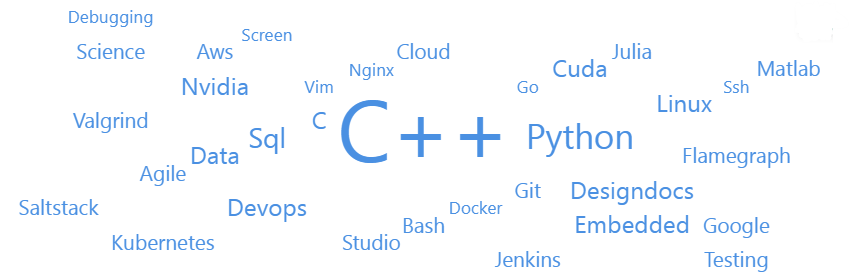
\includegraphics[width=0.99\textwidth]{cloud_long.png}
%\vspace{-4mm}
\end{minipage}
\noindent
\begin{minipage}[t]{0.75\linewidth}
\vspace{-12mm}
\section{Experience}
\cventry{09/2023 - Current}{Growth time}{}{}{}{
\noindent
\begin{minipage}[t]{0.65\textwidth}
Restarted intensive German study. First personal embedded development project (Arduino). Experimented with LLMs, including: prompt engineering, created a CustomGPT to assist with German learning; architecture, discovered the details of transformer structure and parameter efficient training; learnt to run language models locally.
\end{minipage}
}


\cventry{03/2023 - 09/2023 \\ \Company{DoubleCloud} \\ Company size: 50-100}{Software Developer}{}{Zürich}{}{
\noindent
\begin{minipage}[t]{0.65\textwidth}
Maintained and developed the infrastructure around managed ClickHouse, in particular:
\begin{itemize}
\setlength\itemsep{-0.3em}
\item Secured metrics server by adding Nginx
\item Improved SaltStack configuration
\item Solved bugs in Telegraf Go plugins
\end{itemize}
\end{minipage}
}

\cventry{10/2022 - 02/2023}{Personal Time}{}{}{}{
\noindent
\begin{minipage}[t]{0.65\textwidth}
Got married, organized celebrations across two continents. Moved house. Started studying German intensively. Sailed for a week for the first time. Decided to take Data Science certification (see Education). 
\end{minipage}
}

\cventry{06/2021 - 09/2022 \\ \Company{Firebolt} \\ Company size: 50-100}{Software Developer}{}{Zürich}{}{
\noindent
\begin{minipage}[t]{0.65\textwidth}
Maintained and developed the SQL optimization engine and testing infrastructure.
\begin{itemize}
\setlength\itemsep{-0.3em}
\item Expanded supported SQL syntax and optimizations
\item reworked the test framework to support new test suite
\item contributed to rewriting to higher standards the optimization engine 
\end{itemize}
\end{minipage}
}

\cventry{08/2020 - 02/2021 \\ \Company{F-Trust} \\ Company size: 5}{Developer / Analyst}{}{Zug}{}{
\noindent
\begin{minipage}[t]{0.65\textwidth}
\begin{itemize}
\setlength\itemsep{-0.3em}
\item Maintained and developed a Trading Engine (C++)
\item redesigned, implemented and migrated storage (PostgreSQL)
\item extracted and integrated data from multiple log streams
\item analyzed data to highlight opportunities for improvement (Julia)
\end{itemize}
\end{minipage}
}

\cventry{10/2017 - 05/2020 \\ \Company{Google} \\ Company size: 100.000}{Software Developer}{}{Zürich}{}{
\noindent
\begin{minipage}[t]{0.65\textwidth}
Within Search, productionized an initially experimental tool (C++).
\begin{itemize}
\setlength\itemsep{-0.3em}
\item Improved runtime from days to hours
\item added support for new kinds of data
\item made the results easily visualizable and monitorable
\item made onboarding orders of magnitude faster for most cases
\end{itemize}
\end{minipage}
}

\cventry{04/2016 - 10/2017 \\ \Company{Ascent Software}}{Software Developer}{}{Luqa, Malta}{}{
\noindent
\begin{minipage}[t]{0.65\textwidth}
Bridging from internal API to new device API for automotive.
\end{minipage}
}


\cventry{04/2015 - 04/2016 \\ \Company{Rulex Inc.}/\Company{CNR}}{Junior Developer}{}{Genua, Italy}{}{
\noindent
\begin{minipage}[t]{0.65\textwidth}
Reworked C/MATLAB algorithms for OpenMP/CUDA parallelization
\end{minipage}
}
\end{minipage}
\begin{minipage}[t]{0.25\linewidth}
%\vspace{-13mm}
\fcolorbox{lightorange}{white}{
\begin{tabular}{lc}
\tsection{Languages}
English & Fluent professional \\
Italiano & Madrelingua \\
Deutsch & B1, B2 geplänt 03/24 \\
Français & Bon \\
\end{tabular}
}
\begin{tabular}{lc}
\tsection{Programming}
\tskl{C++}{5}
\tskl{- C++/Abseil}{5}
\tskl{- C++/Boost}{4}
\tskl{SQL}{5}
\tskl{- Clickhouse SQL}{5}
\tskl{- PostgreSQL}{4}
\tskl{Python}{4}
\tskl{Julia}{2}
\tskl{Go}{1}
\tsection{Tools}
\tskl{BASH}{4}
\tskl{Linux}{4}
\tskl{Windows}{3}
\tskl{Visual Studio}{2}
\tskl{AWS storage}{2}
\tskl{Docker}{3}
\tskl{Git}{5}
\tskl{Jenkins CI}{3}
\tskl{SSH}{3}
\tskl{VIM}{3}
\tskl{Valgrind}{3}
\tskl{Flamegraph}{2}
\tskl{Nvidia CUDA}{2}
\tskl{OpenMP}{3}
\tsection{Competences}
\tskl{Testing}{5}
\tskl{Debugging}{4}
\tskl{DevOps}{4}
\tskl{Design Docs}{5}
\tskl{Embedded Dev.}{1}
\tskl{Agile Dev.}{4}
\end{tabular}
\end{minipage}

\pagebreak

\section{Formal education}

\cventry{2023 H1}{\href{https://execed-online.imperial.ac.uk/business-analytics}{Business Analytics: From Data to Decisions}}{Imperial College Business School}{}{}{}
\cventry{2009--2015}{\href{http://www.unipd-scuolagalileiana.it/en/}{Galileian School of Higher Education}}{University of Padua}{University-level enriching program for gifted students}{\textit{98/100}}{}
\cventry{2012--2014}{Master Degree in Mathematics}{University of Padua}{}{\textit{108/110}}{}
\cventry{2009--2012}{Bachelor Degree in Mathematics}{University of Padua}{}{\textit{110/110 cum Laude}}{}
\cventry{2004--2009}{High School - Science Track, added IT, French}{Liceo Fermi}{Bologna}{\textit{100/100 cum Laude}}{}

\newcommand{\BeginCourses}{%
	\begin{tabular}{r@{\hspace{1em}}c@{\hspace{1em}}p{0.5\textwidth}}
}
\newcommand{\EndCourses}{\end{tabular}}

\newcommand{\Course}[3]{%
\hspace{1.5em} #1 & \textit{#3} & \textbf{#2} \\
}


\section{Continuous Learning}

\subsection{Data Science/Analytics}
\columnratio{0.72}
\begin{paracol}{2}
\switchcolumn[0]*
\BeginCourses
\Course{Nov 2023}{Data Fluency: Exploring and Describing Data}{Linkedin}
\Course{Nov 2023}{Power BI Essential Training}{Linkedin}
\Course{Oct 2023}{Business Intelligence for Consultants}{Linkedin}
\Course{Oct 2023}{Data Analytics for Business Professionals}{Linkedin}
\Course{Oct 2023}{Excel: Economic Analysis and Data Analytics}{Linkedin}
\Course{Oct 2023}{The Non-Technical Skills of Effective Data Scientists}{Linkedin}
\EndCourses
\switchcolumn
\begin{tabular}{p{3cm}c}
\tskl{Data Analysis}{3}
\tskl{Data Visualization}{4}
\tskl{Probability}{4}
\tskl{Microsoft Power BI}{2}
\tskl{Microsoft Excel}{5}
\tskl{Pandas}{4}
\end{tabular}
\end{paracol}

\subsection{AI and LLMs}

\subsection{Programming languages}
\begin{paracol}{2}
\BeginCourses
\Course{Nov 2023}{\Csh Essential Training 1: Types and Control Flow}{Linkedin}
\Course{Oct 2023}{Learning MATLAB}{Linkedin}
\EndCourses
\switchcolumn
\begin{tabular}{p{3cm}c}
\tskl{\Csh}{2}
\tskl{MATLAB}{3}
\end{tabular}
\end{paracol}

\subsection{Embedded development}
\begin{paracol}{2}
\BeginCourses
\Course{Nov 2023}{C Programming for Embedded Applications}{Linkedin}
\EndCourses
\switchcolumn
\begin{tabular}{p{3cm}c}
\tskl{C Embedded}{3}
\end{tabular}
\end{paracol}
\subsection{Cloud and DevOps}
\begin{paracol}{2}
\BeginCourses
\Course{Feb 2023}{AWS Certified Solutions Architect - Associate (SAA-C02) Cert Prep: 1 Cloud Services Overview}{Linkedin}
\Course{Jan 2023}{DevOps Foundations: Going Cloud Native}{Linkedin}
\EndCourses
\switchcolumn
\begin{tabular}{p{3cm}c}
\tskl{Cloud Admin}{3}
\tskl{AWS Cloud}{4}
\tskl{DevOps}{3}
\end{tabular}
\end{paracol}

\newcommand{\Project}[5]{
\hspace{-1em}\raisebox{\dimexpr\ht\strutbox-\height}{\includegraphics[width=0.12\textwidth]{#1}} & #2 & \textbf{#3} \newline \href{http://#4}{\textcolor{blueGray}{#4}} \newline #5 \\ 
}

\section{Projects}

\subsection{Embedded}
\begin{paracol}{2}
\BeginCourses
\Project{arduino_btc_project.jpg}{Nov 2023}{BTC Arduino monitor}{github.com/Fdondi/arduino-btc}{A bot checking Bitcoin prices and blinking a green led if the price is above average, red if below. The speed of blinking depends on the magnitude of the change.}
\EndCourses
\switchcolumn
\begin{tabular}{p{3cm}c}
\tskl{C++ Embedded}{3}
\tskl{Arduino}{2}
\tskl{SSH embedded}{1}
\tskl{Embedded Development}{2}
\end{tabular}
\end{paracol}

\subsection{LLMs / Prompt engineering}
\begin{paracol}{2}
\BeginCourses
\Project{worterbuch.png}{Dec 2023}{Deutsches Wörterbuch}{chat.openai.com/g/g-bpvvdzIKE-deutsches-worterbuch}{A CustomGPT, takes one word and provides grammar, explanation in German and English, examples of use, and a final image visualizing the concept. Clarifies ambiguous or misspelled words, can discuss any user doubt. Can adjust German level used both automatically and on request.}
\EndCourses
\switchcolumn
\begin{tabular}{p{3cm}c}
\tskl{AI UX}{3}
\tskl{Prompt engineering}{3}
\end{tabular}
\end{paracol}

\subsection{UI/Design}
\begin{paracol}{2}
\BeginCourses
\Project{CV.png}{Dec 2023}{This CV}{github.com/Fdondi/cv-latex}{\LaTeX CV, heavily modified from \textit{moderncv}, with a wordcloud and second bar on the left to showcase competences level. Two more colors introduced. Courses and projects are diplayed with custom formatting.}
\EndCourses
\switchcolumn
\begin{tabular}{p{3cm}c}
\tskl{\LaTeX}{5}
\tskl{Business communication}{4}
\end{tabular}
\end{paracol}

\end{document}
